\documentclass[11pt]{article}
\usepackage[margin=1in]{geometry}
\usepackage{graphicx}
\usepackage{amsmath}
\usepackage{booktabs}
\title{Spectral MP Audit}
\date{}
\begin{document}
\maketitle

\section*{Problem statement}
We test whether the top eigenvalue of the observed matrix exceeds the Marchenko--Pastur (MP) bulk edge, consistent with a spike outside random-matrix noise.

\section*{Definitions}
Let $q=N/T$. The MP upper edge is
\[
\lambda_+ = \sigma^2(1+\sqrt{q})^2.
\]
For correlation-like matrices, $\sigma^2=1$.

\section*{Data and parameter extraction}
\begin{itemize}
\item Matrix $C$ path: \texttt{/Users/mathieujonathan/Desktop/quantum-liram-research/chatgpt_exports/2026-02-16/artifacts/2026-02-16/reports/layer_correlation_matrix.csv}
\item $N=37$, $T=108$, $q=0.342593
\item Correlation-like: \texttt{True} (diag mean = 1.000000)
\item $\sigma^2=1.000000$
\end{itemize}

\section*{Results}
\begin{itemize}
\item Observed $\lambda_1 = 8.726491$
\item MP edge $\lambda_+ = 2.513221$
\item $\Delta_1=\lambda_1-\lambda_+ = 6.213270$
\item Empirical null p-value: $p_{emp}=0.00199601$ using $M=500$ (column_permutation_null)
\end{itemize}

\section*{Empirical Monte Carlo method}
If an $X$ matrix is available, each column is independently permuted (after standardization) to generate null samples; otherwise, Gaussian synthetic null matrices are used under MP assumptions. For each null sample, the top eigenvalue is computed.

\section*{Figures}
\begin{figure}[h!]
\centering
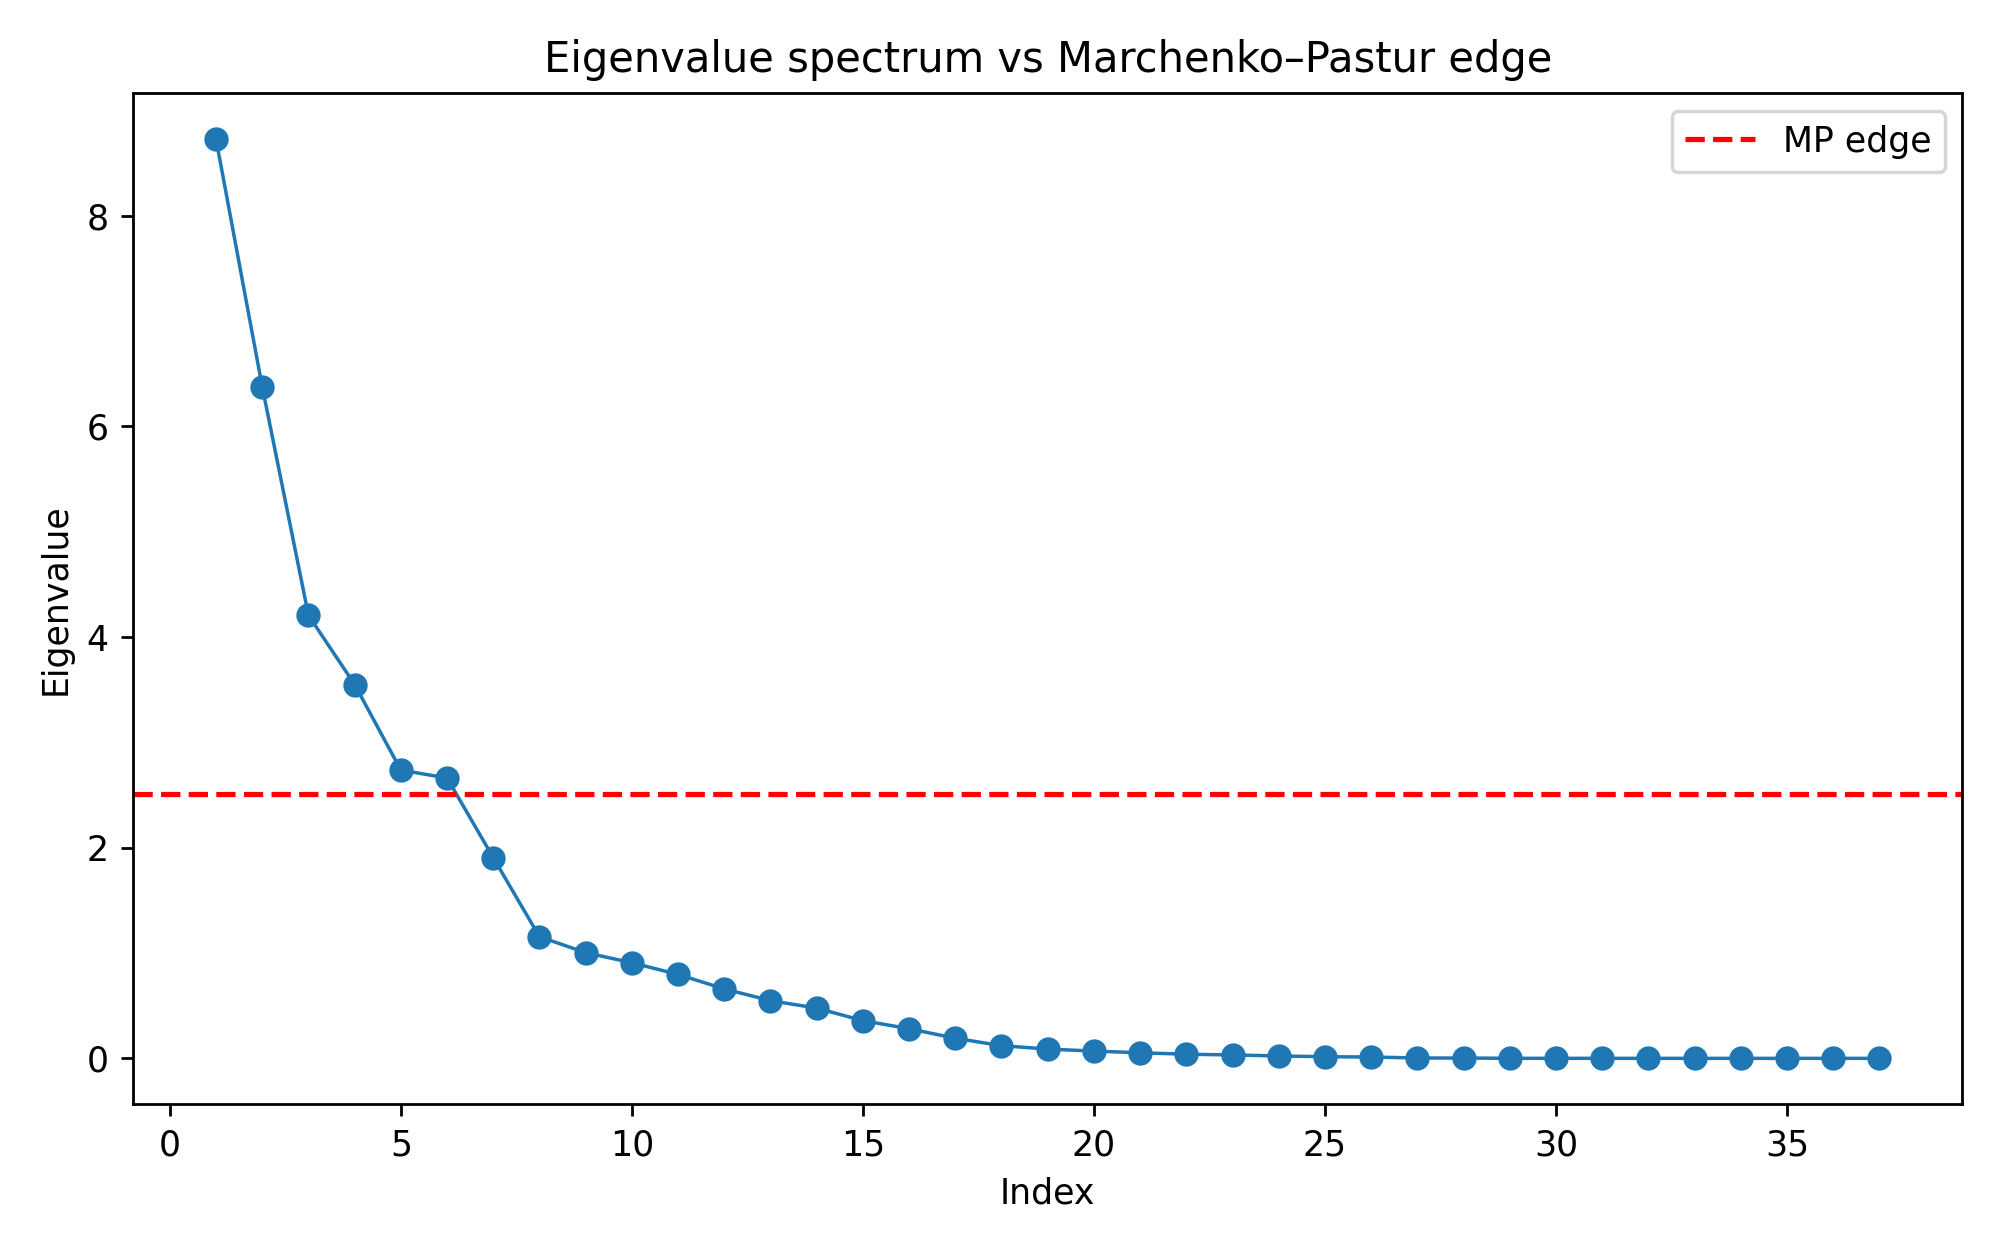
\includegraphics[width=0.85\textwidth]{figures/eigen_spectrum_vs_mp.png}
\caption{Eigenvalue spectrum vs MP edge.}
\end{figure}

\begin{figure}[h!]
\centering
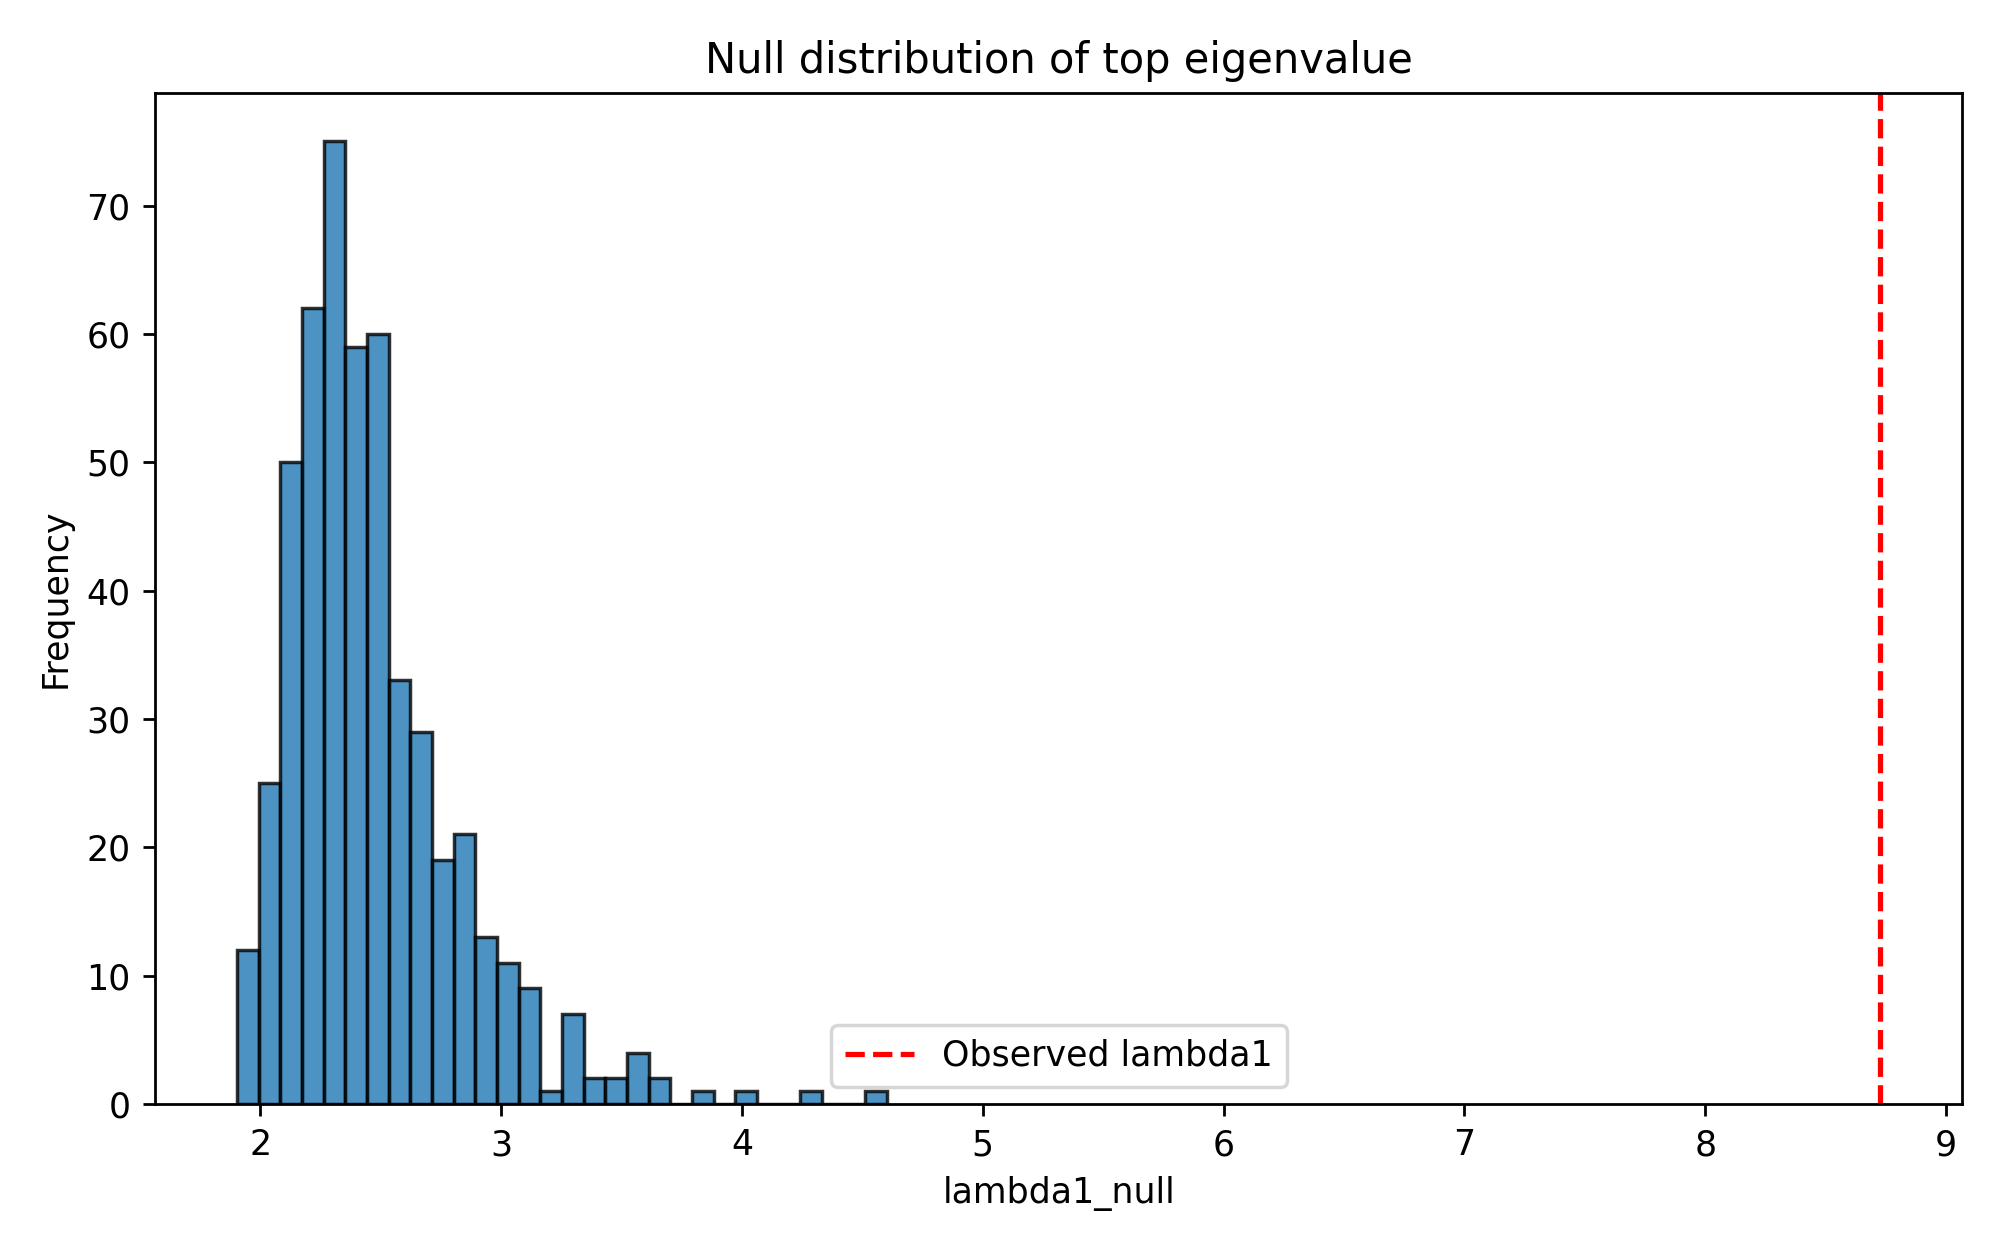
\includegraphics[width=0.85\textwidth]{figures/lambda1_null_hist.png}
\caption{Null distribution of top eigenvalue with observed value.}
\end{figure}

\end{document}
